\documentclass[12pt]{article}
\usepackage[a4paper,margin=1in]{geometry}
\usepackage{amsmath, amssymb}
\usepackage{listings}
\usepackage{graphicx,float}
\usepackage{hyperref}

\title{AMS 595 - Assignment 7}
\author{Amol Arora, SBUID: 116491705}
\date{December 15, 2024}

\begin{document}

\maketitle

\section*{1. Work Done}
\underline{Github Link for the Project}: \url{https://github.com/amol1202/AMS595-Assignment7} \\[8pt]
This project involved implementing various programming tasks in C++ based on the given requirements. The main tasks included:

\begin{enumerate}
    \item Translating MATLAB conditional statements to C++.
    \item Implementing a function to print vectors.
    \item Generating Fibonacci numbers using a \texttt{while} loop.
    \item Writing functions for:
    \begin{itemize}
        \item Checking if a number is prime.
        \item Finding the factors of a number.
        \item Prime factorization of a number.
    \end{itemize}
    \item Printing the first \(n\) rows of Pascal's Triangle using recursion or iteration.
\end{enumerate}
\hrule
\section*{2. Implementation}
Each task was implemented in C++ with proper comments and structured code.

\subsection*{Task 1: Conditional Statements}
The MATLAB conditional statement was translated into a C++ \texttt{switch} statement. This allows efficient handling of discrete cases.

\subsection*{Task 2: Printing a Vector}
A custom function \texttt{print\_vector} was created to iterate over and print all elements of a vector.

\subsection*{Task 3: Fibonacci Sequence}
Using a \texttt{while} loop, the Fibonacci sequence was generated for terms not exceeding 4,000,000.

\subsection*{Task 4: Prime, Factorization, and Prime Factorization}
Functions for determining primality, finding factors, and performing prime factorization were implemented using loops and conditionals. Test cases validated correctness.

\subsection*{Task 5: Pascal's Triangle}
Pascal's Triangle was generated row by row, with calculations based on the binomial coefficient formula.
\vspace{6pt}
\hrule
\section*{3. Results}

The following outputs were obtained for the respective tasks:

\subsection*{Task 1: Conditional Statements}
\textbf{Input:} \texttt{-1} \newline
\textbf{Output:} \texttt{negative one}

\subsection*{Task 2: Printing a Vector}
\textbf{Input:} \texttt{\{1, 2, 3, 4\}} \newline
\textbf{Output:} \texttt{1 2 3 4}

\subsection*{Task 3: Fibonacci Sequence}
\textbf{Output:} Fibonacci numbers up to 4,000,000: \newline
\texttt{1 2 3 5 8 13 21 34 55 ...}

\subsection*{Task 4: Prime and Factorization}
\textbf{Test Cases for Prime Check:} \newline
\texttt{is\_prime(2) = true, is\_prime(10) = false, is\_prime(17) = true} \\[8pt]
\textbf{Test Cases for Factorization:} \newline
\texttt{Factors of 72: 1 2 3 4 6 8 9 12 18 24 36 72} \\[8pt]
\textbf{Test Cases for Prime Factorization:} \newline
\texttt{Prime factors of 72: 2 2 2 3 3}

\subsection*{Task 5: Pascal's Triangle}
\textbf{Output for 5 rows:}
\begin{verbatim}
1
1 1
1 2 1
1 3 3 1
1 4 6 4 1
\end{verbatim}
My results after compiling and running the code in command prompt $\longrightarrow$
\begin{figure}[H]
    \centering
    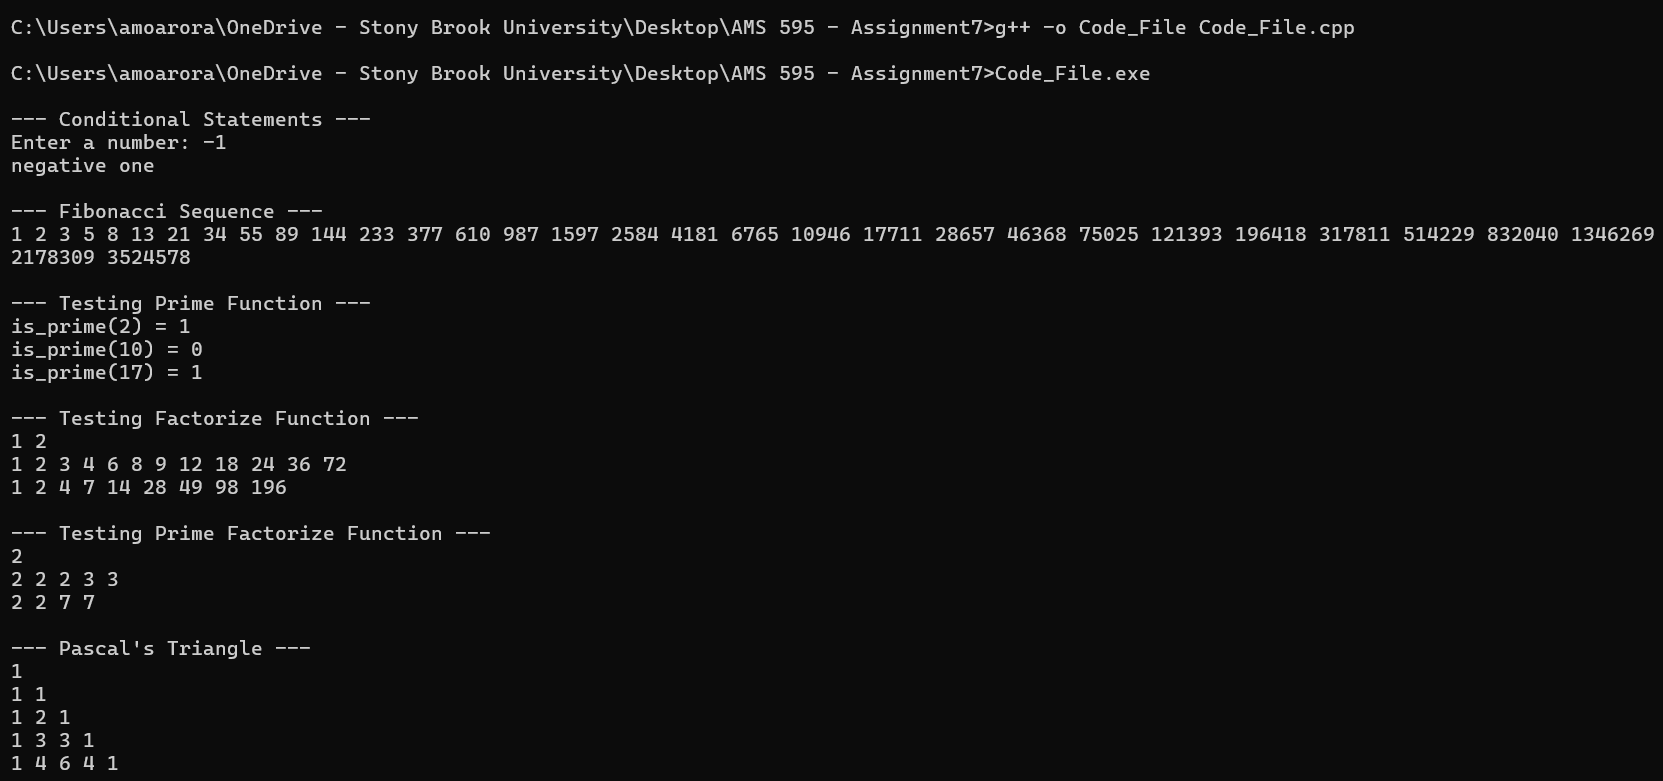
\includegraphics[width=1.13\textwidth]{results.png}
    \caption{Results in command prompt}
    \label{fig:results}
\end{figure}
\hrule
\section*{4. How to Run the Code}
\begin{enumerate}
    \item Ensure a C++ compiler (e.g., g++) is installed on your system.
    \item Save the provided source code as \texttt{project.cpp}.
    \item Compile the code using the command: \newline
    \texttt{g++ -o project project.cpp}
    \item Run the executable using the command: \newline
    \texttt{./project}
\end{enumerate}
\hrule
\section*{5. Conclusion}
This project provided hands-on experience with fundamental C++ concepts, including conditional statements, loops, functions, and recursion. The implementation was verified against test cases to ensure correctness.
\vspace{6pt}
\hrule
\end{document}